\BiChapter{基于视角增强的光场显著性目标检测}{TODO}
\label{chap:part4}
%
%
%
%
第三章从焦点感知的角度出发,设计了一种切片级探索多视角场景聚焦信息的显著性目标检测算法。
该方法注重对多视角三维场景的感知,以及不同视角对显著性预测的贡献程度,
实现了光场信息的深度挖掘以及多视角信息的高效探索。
%
%
本章从视角强化的角度出发,基于注意力机制引入视角增强模块,并通过前背景的补偿模块优化网络的训练,
实现了光场信息的充分挖掘。
%
%
%
%
\BiSection{研究动机}{TODO}
%
%
%
%
光场技术可以完整地记录场景的几何信息。在其中,焦点堆栈数据是光场数据的关键表达形式之一。现有研究表明,光场数据在显著性目标检测方面具有优势。
随着基于Transformer架构的模型在各种视觉任务上取得超越性的性能,基于Transformer架构的光场显著性检测网络也逐渐出现\cite{wang2023tenet,liu2023lftransnet}。
然而,直接应用Transformer架构到光场显著性检测任务中,
并不能充分发挥Transformer架构对于长距离建模的能力,
不能得到理想的光场显著性目标检测效果。
还要设计合适的网络结构,加强模型对光场中隐含空间场景的感知,
来使得模型对光场显著性检测有一个鲁棒性的结果。
%
%
%
%
\par
\begin{figure}[!ht]
	\centering
	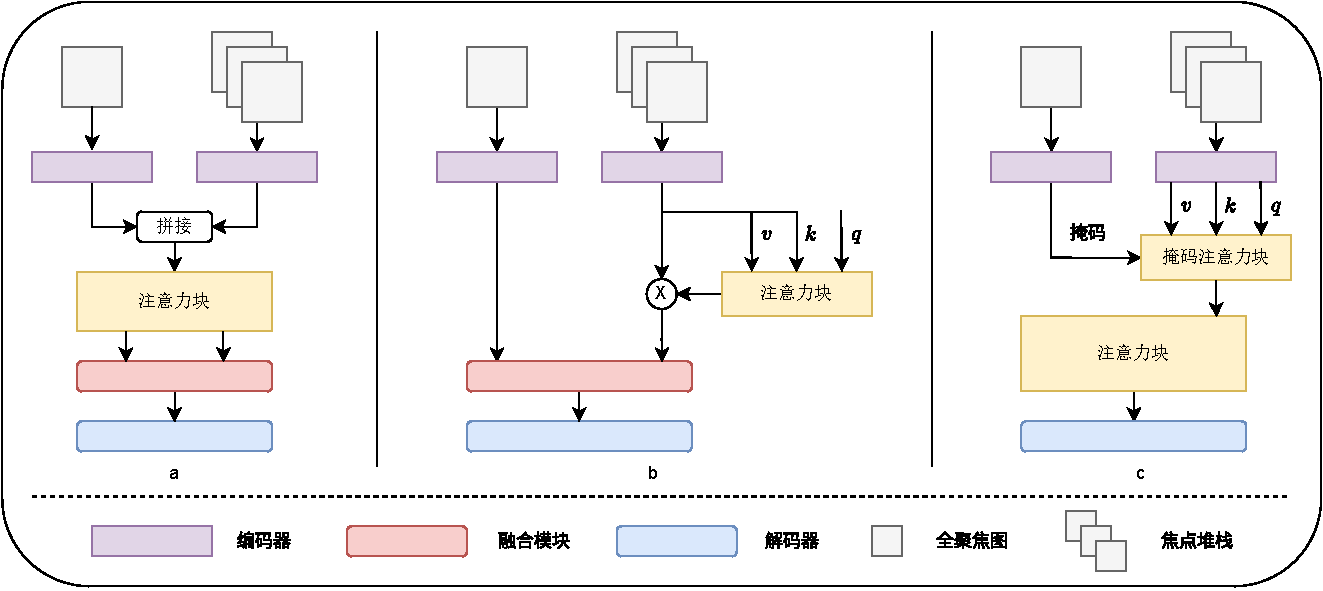
\includegraphics[width=0.95\linewidth]{figures/chapter4/task2_ins.drawio}
	\bicaption{光场模型范例}{TODO}  
	\label{cpt4_fig1:task2_ins}
\end{figure}
%
%
%
%
王等人~\cite{wang2023tenet}通过拼接焦点堆栈和全聚焦图特征,
一并送入Transformer编码器来,建立光场整体结构的感知模型。
如图~\ref{cpt4_fig1:task2_ins}~(a)~所示,
但是这种方式弱化了全聚焦图片特征和散焦图片特征之间的模态差异,两个模态之间的融合依然依赖后续的融合模块。
刘等人~\cite{liu2023lftransnet}只在焦点堆栈支路使用了Transformer结构。该方法聚合多尺度的焦点堆栈特征构造注意力矩阵,用一个可学习的权重来作为查询矩阵。通过注意力运算来汇总不同切片对显著性检测的贡献。如图~\ref{cpt4_fig1:task2_ins}~(b)~所示。
%
%
但是,这些方法没有充分考虑两个模态之间的差异,融合方式有限,起到的特征强化效果也有限。


针对上述问题,本章提出来一种基于视角增强的光场显著性目标检测方法。
此方法致力于从焦点堆栈和全聚焦图的差异入手,结合Transformer强大的注意力机制,提出了合成增强视角的注意力方法。


~

随着



然而,采集光场数据需要多组摄像头或相机矩阵,造成了高昂的成本。为了实现理想的光场显著性目标检测能力,除了设计合适的网络模型外,还需要大量高质量的光场数据。由于光场数据获取成本高,目前的方法通常采用数据增强手段来增加训练数据。传统的数据增强方法包括旋转、平移、裁剪和缩放等操作,但这些方式的变化有限,效果也不够显著。对于不同类型的光场数据,需要不同的增强方法,选择不当的方法可能会引入噪声,导致训练不稳定,降低模型性能。因此,如何稳定生成高质量的光场数据以实现数据增强的目标是当前需要解决的问题。



针对上述问题。  
  
为验证本方法的有效性,本章在 DUT-LFSD, LFSD 以及 HFUT-LFSD
数据集上进行了实验,同样获得了超越传统数据增强手段的性能,为光场数据的应用奠
定了基础。为了进一步验证本方法的有效性,本章将提出的数据增强方法应用在当前最
好的光场显著性检测方法上,实验结果表明,本章的数据增强方法能够提升其它方法的
检测性能。



% task2_ins.drawio


\BiSection{方法介绍}{TODO}





%
%
%
%
\BiSubsection{视角增强模块}{TODO}

\BiSubsection{感知学习策略}{TODO}

\BiSubsection{训练过程}{TODO}


%\\
%\\
%\\
%\\
\BiSection{实验结果与分析}{TODO}

\BiSubsection{实验设置}{TODO}

\BiSubsection{消融实验}{TODO}

\BiSubsection{对比实验}{TODO}


%\\
%\\
%\\
%\\
\BiSection{本章总结}{TODO}